\section{Operation of timed functions}
\label{sec:libinger}

%Figure~\ref{fig:architecture} shows a dependency graph of the software
%components that implement preemptible functions (rectangular boxes), their
%relationship to the existing runtime environment (hexagonal box), and the
%points at which third-party code can use our abstractions (ovals).
%
%This section describes the components  detail.  We start by discussing
%\textit{libinger}, a library that provides the preemptible function abstraction
%(Section~\ref{sec:libinger}).  Next, we present our experience porting a userland
%threading library to libinger in order to make its scheduler preemptive
%(Section~\ref{sec:threading}).  We then explain \textit{libgotcha}, a supporting
%library that automatically addresses many problems related to shared state in
%third-party code (Section~\ref{sec:libgotcha}).  Finally, we illustrate the
%significance of libgotcha by demonstrating its ability to provide POSIX async-signal
%safety in places where it would not otherwise exist (Section~\ref{sec:statefulness}).
%
%
%
%\begin{figure}
%\begin{center}
%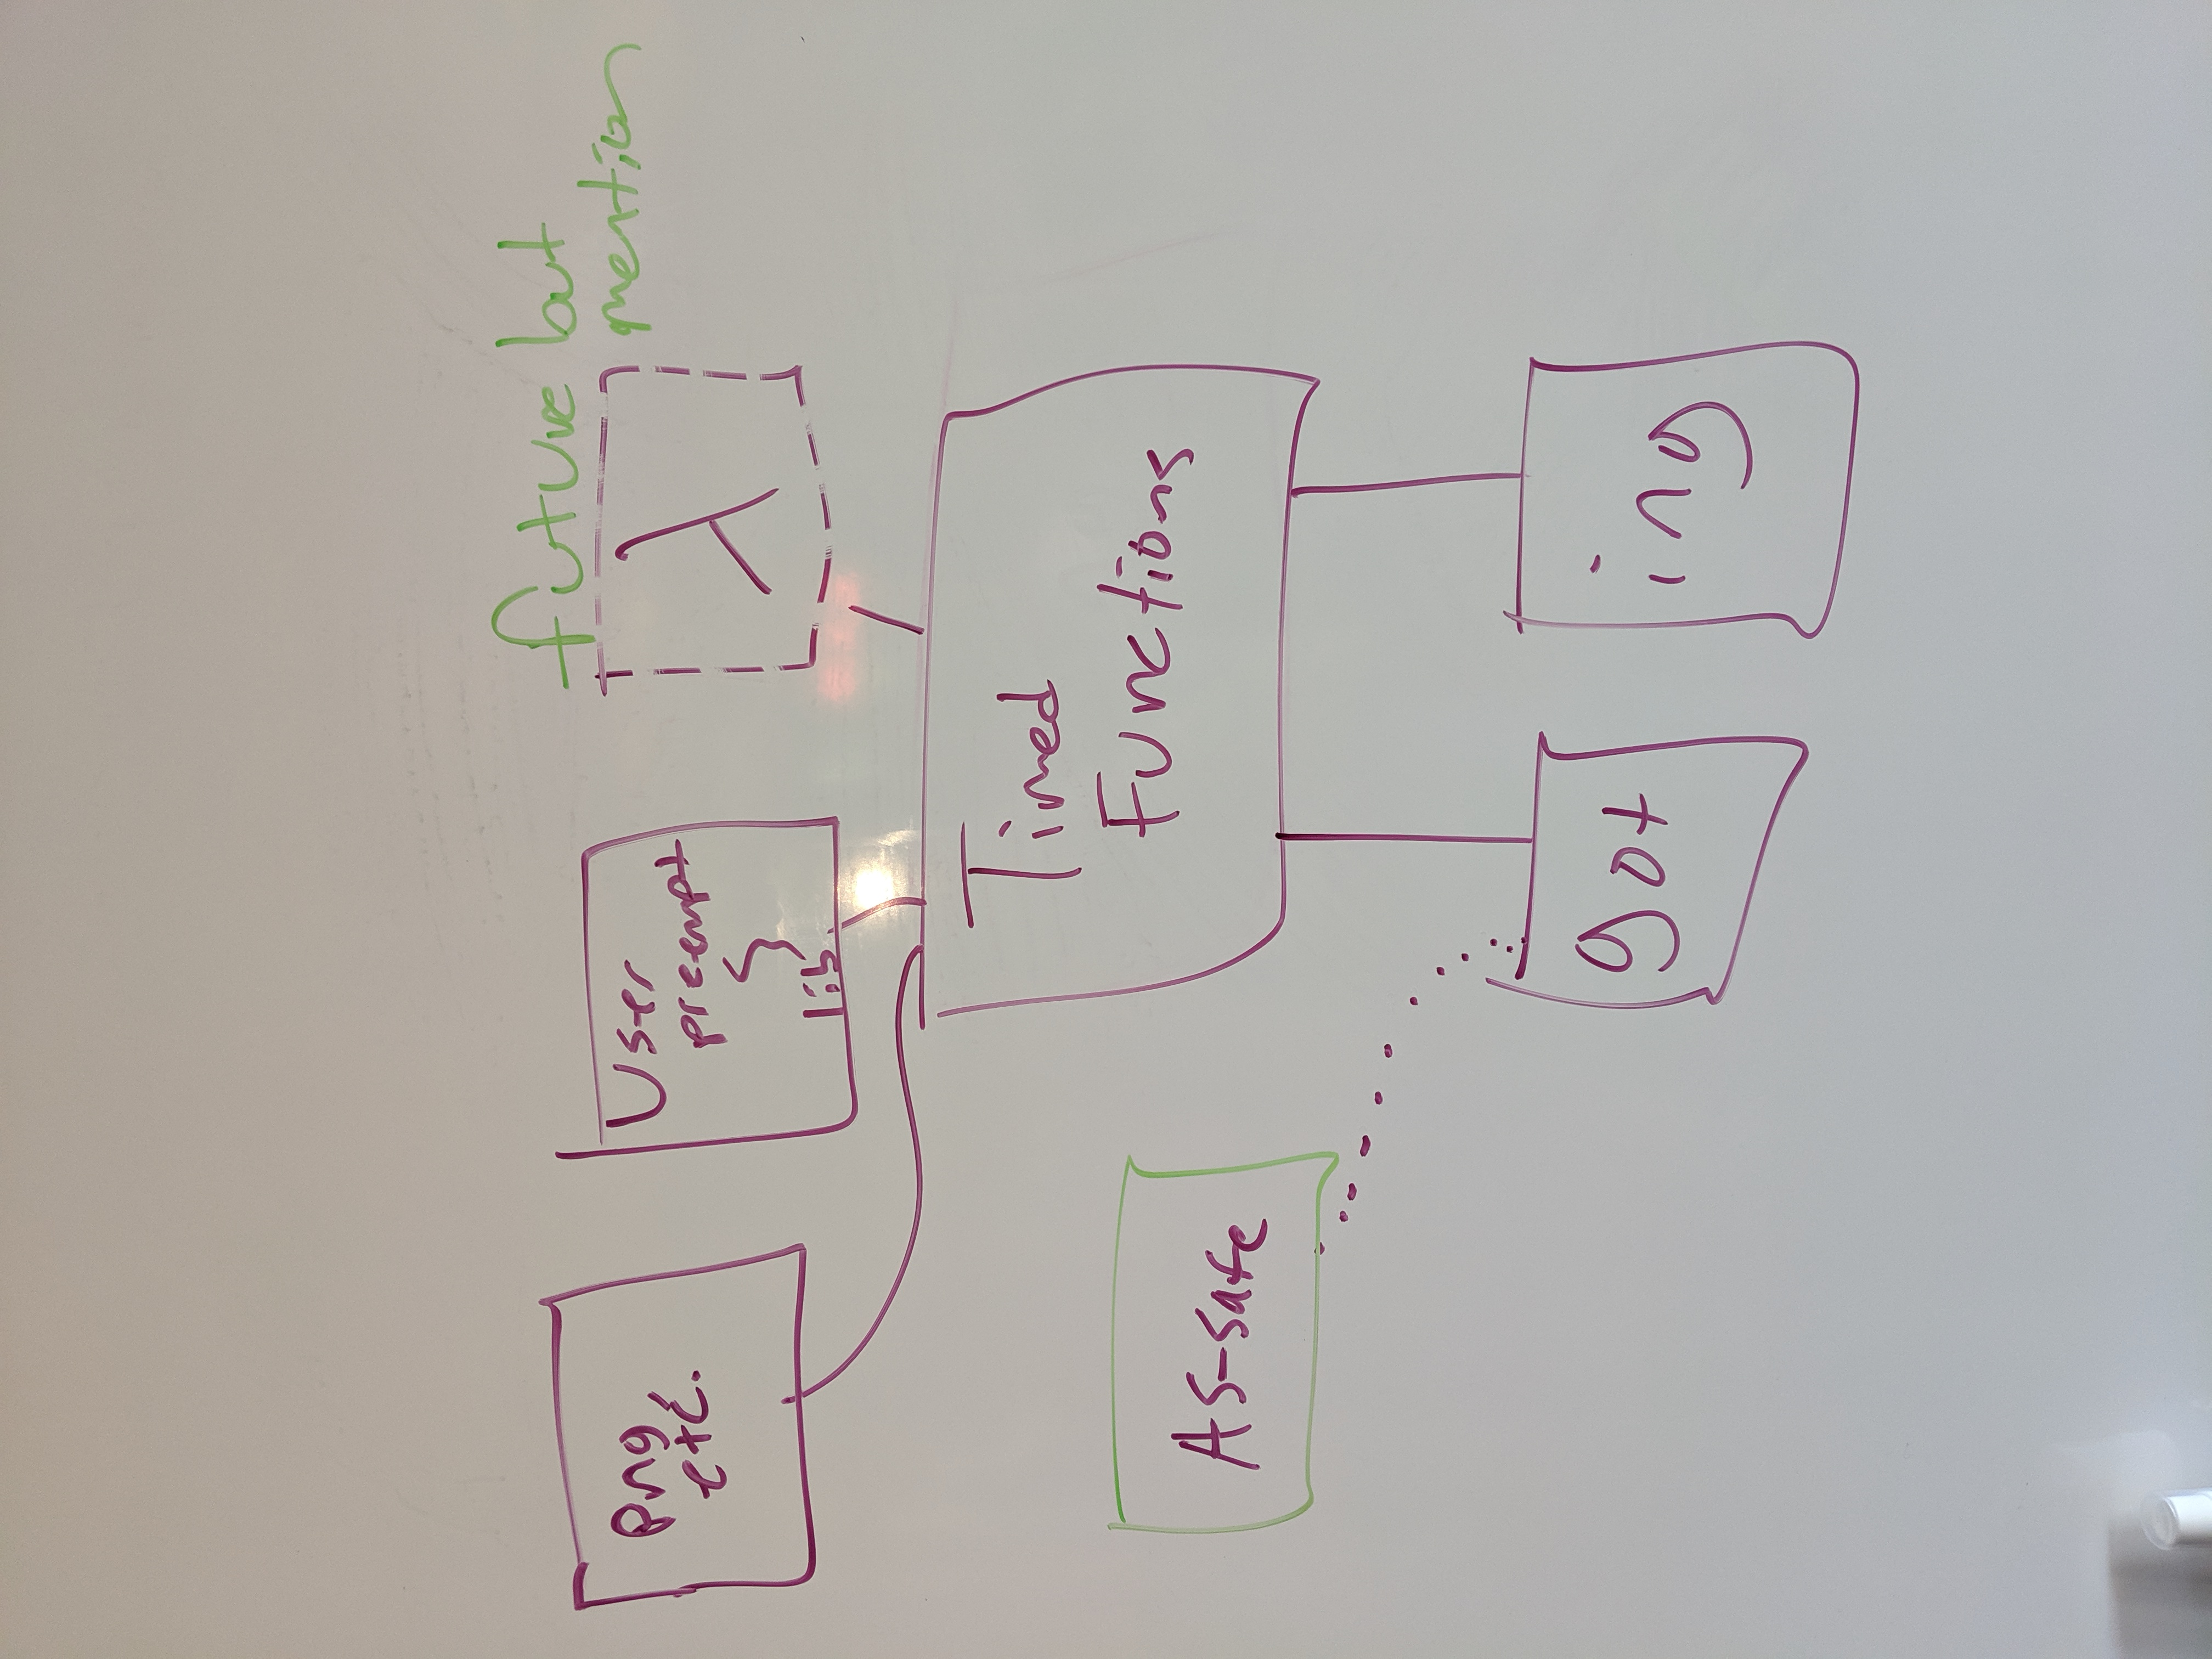
\includegraphics[width=0.75\columnwidth]{figs/architecture}
%\end{center}
%\caption{The preemptible functions stack}
%\label{fig:architecture}
%\end{figure}

The \textit{libinger} library implements the preemptible function interface. Although
it provides users with the familiar function call interface, internally,
\textit{libinger} uses a combination of unstructured control flow in the form of
multiple stack regions and signal handlers. \textit{libinger} runs each timed
function on a separate stack, different from the user's own stack. This is
necessary to prevent different functions or the user from clobbering each
other's stack when some timed functions have been preempted.

\subsection{Timer interrupts}


\begin{figure}
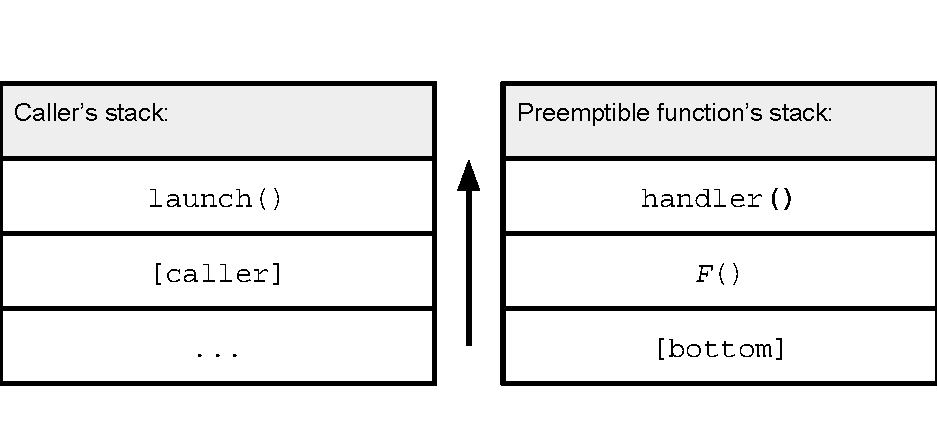
\includegraphics[width=\columnwidth]{figs/twostacks}
\caption{The stacks before and after a timeout.  \textnormal{Upon discovering
that the preemptible function has exceeded its time bound, the handler returns to the
checkpoint continuation within the \texttt{launch()} function, removing its own stack
frame in the process.  Then, \texttt{launch()} returns to the original call site,
which removes its stack frame.}}
\label{fig:twostacks}
\end{figure}

While \textit{libinger} is executing a executing the user-provided function, we
enable fine-grained timer interrupts to periodically run our signal handlers
that monitor the execution of the preemptible functions. While a preemptible
function is running, the timer interrupt fires periodically, causing the signal
handler to be invoked each time. If a function exceeds its timeout, \textit{libinger}
jumps back to the caller, returning a continuation that stores the preemptible
function's register values.

Figure~\ref{fig:twostacks} shows the two stacks of execution, belonging to the
\textit{libinger} user and the preemptible function, present while the signal handler
is running. It also shows what happens to the stack frames of both if the
function times out. The handler first checks whether the preemption signal was
intended for the current thread, as described earlier.  It then checks whether
the preemptible function has exceeded its timeout; if so, it swaps the contents
of the signal handler's continuation (accessible via the final argument to the
function~\cite{sigaction-manpage}) with the checkpoint continuation saved by
\texttt{launch()}.  This causes the subsequent return from the signal handler
to jump back to \texttt{launch()}, which then returns a \texttt{linger}
structure containing the signal handler's original context.  A subsequent
\texttt{resume()} call on this packaged continuation proceeds in much the same
way as \texttt{launch()}, but resumes the original computation by sending
itself a special signal with \texttt{pthread\_kill()}, then swapping the saved
context with the contents of that handler's context\footnote{This is necessary
because POSIX left the semantics of calling \texttt{setcontext()} on the
continuation saved by a signal handler invocation unspecified, leading
implementations such as GNU not to handle this
case~\cite{getcontext-manpage}.}.

When the caller is finished with a preemptible function, it must deallocate it
either explicitly (C) or implicitly via the \texttt{inger} type's destructor
(Rust).  This cleans up the \textit{libinger} resources allocated by
\texttt{launch()};
however, if the call constitutes a cancellation, the current implementation of
\textit{libinger} does not automatically clean up resources already allocated by the
preemptible function itself.  While the lack of a standard deinitialization API
makes this inherently hard to do in C, it is possible to implement in languages
such as Rust that support destructors.  For instance, the approach proposed by
Boucher et al.~\cite{boucher:atc2018} could be employed to raise a panic
(exception) on the preemptible function's stack, causing the language runtime
to unwind each stack frame, invoking the destructor of each local variable in
the process.


\subsection{Performance goals}

Although seeking to implement low-latency preemption without requiring a custom
operating system, we sought a design that could operate with performance
comparable to Shinjuku's.  Our prototype is not yet optimized to this extent,
but we provide a back of the envelope calculation of its minimum possible
preemption latency based on Shinjuku's comparison of the latency of bare-metal
interprocessor interrupts (IPIs) versus Linux signals (measured from their
request by one core to the invocation of the other's interrupt service routine
or signal handler).  While IPIs take an average of only 1993 cycles, compared
to 4950 for signals (a ratio of 1:2.5), a look at their sender/receiver
breakdown of the latter number suggests two opportunities to reduce this
overhead without abandoning the existing systems software stack:  First, 343 of
those cycles (6.9\%) are spent propagating the signal between the two cores,
and should largely disappear by initiating it on the same thread that is to be
preempted.  Second, 2084 cycles (42\%) are incurred by the sender, of which
some portion should also disappear~\cite{Kaffes:nsdi2019}.  We therefore expect
that an optimized system based on intra-thread signals built atop the existing
system stack could achieve an average preemption latency within 2.5x of that of
their custom operating system with a dedicated watchdog core.


\subsection{Case study: Userland threading}
\label{sec:threading}
